\documentclass[11pt]{extarticle}
\usepackage[utf8]{inputenc}
\usepackage{cite}
\usepackage{graphicx}

% Fontsize of figure smaller than normalsize:
\usepackage{caption}
\captionsetup[figure]{font=small}
\captionsetup[table]{font=small}

\usepackage{pgfplots}
\pgfplotsset{compat=1.16}

\title{Planar Monocular SLAM}
\author{Michele Cipriano}
\date{\today}

\begin{document}

\maketitle

\section{Introduction}
The aim of the project is to develop a full SLAM system capable of determining
the trajectory followed by a robot when moving in an environment with a
representation of the environment itself (the map consisting of the landmarks).
In particular, the program has to work with an initial guess of the trajectory
given by the odometry and an image for each of the pose of the robot in the
trajectory itself. The image (actually a simplified data structure
containing for each seen landmark its image coordinates and its appearance)
must be used in order to improve the trajectory and build the map of the
environment.

The approach followed is a total least squares method, integrating pose-pose
constraints given by the odometry and pose-landmark constraints given by
each image. Before executing the least squares algorithm, the position of each
landmark is initialized with a Direct Linear Transformation (DLT) algorithm.
Each landmark is associated to a certain landmark depending on its appearance
using a k-d tree, which has been initialized with the appearance of all the
landmarks of the map (hence simplifying the problem of updating the k-d
tree depending on all the measurements).

The program, entirely written in C++, manages to correctly find the right
trajectory, making it correspond exactly with the ground truth. The
landmarks are correctly reconstructed as well, with the exception of
a small fraction which did not converge to the right position due to a bad
initialization.

\section{Landmark Initialization}
As introduced in the previous section, the position of each landmark is
initialized with the DLT algorithm, following the analysis discussed in
\cite{Hartley2004}. The data available in the dataset allow to use this
technique which depends only on the homogeneous camera projection matrix of
each pose (initialized with the odometry, the transform between the robot
and the camera and the camera calibration matrix of the dataset). A matrix
is initialized for each landmark with all the measurements from all the
positions in the odometry; then, following Algorithm A5.4 in \cite{Hartley2004},
the position of the landmark is initialized. The initial reconstruction
can be seen in Fig. \ref{fig:dlt-init}.

Note that in this step each measurement
is associated to a certain landmark depending on the data (appearance of the
landmark itself) contained in the k-d tree. If no association can be done
the measurement is discarded.
\begin{figure}
    \centering
    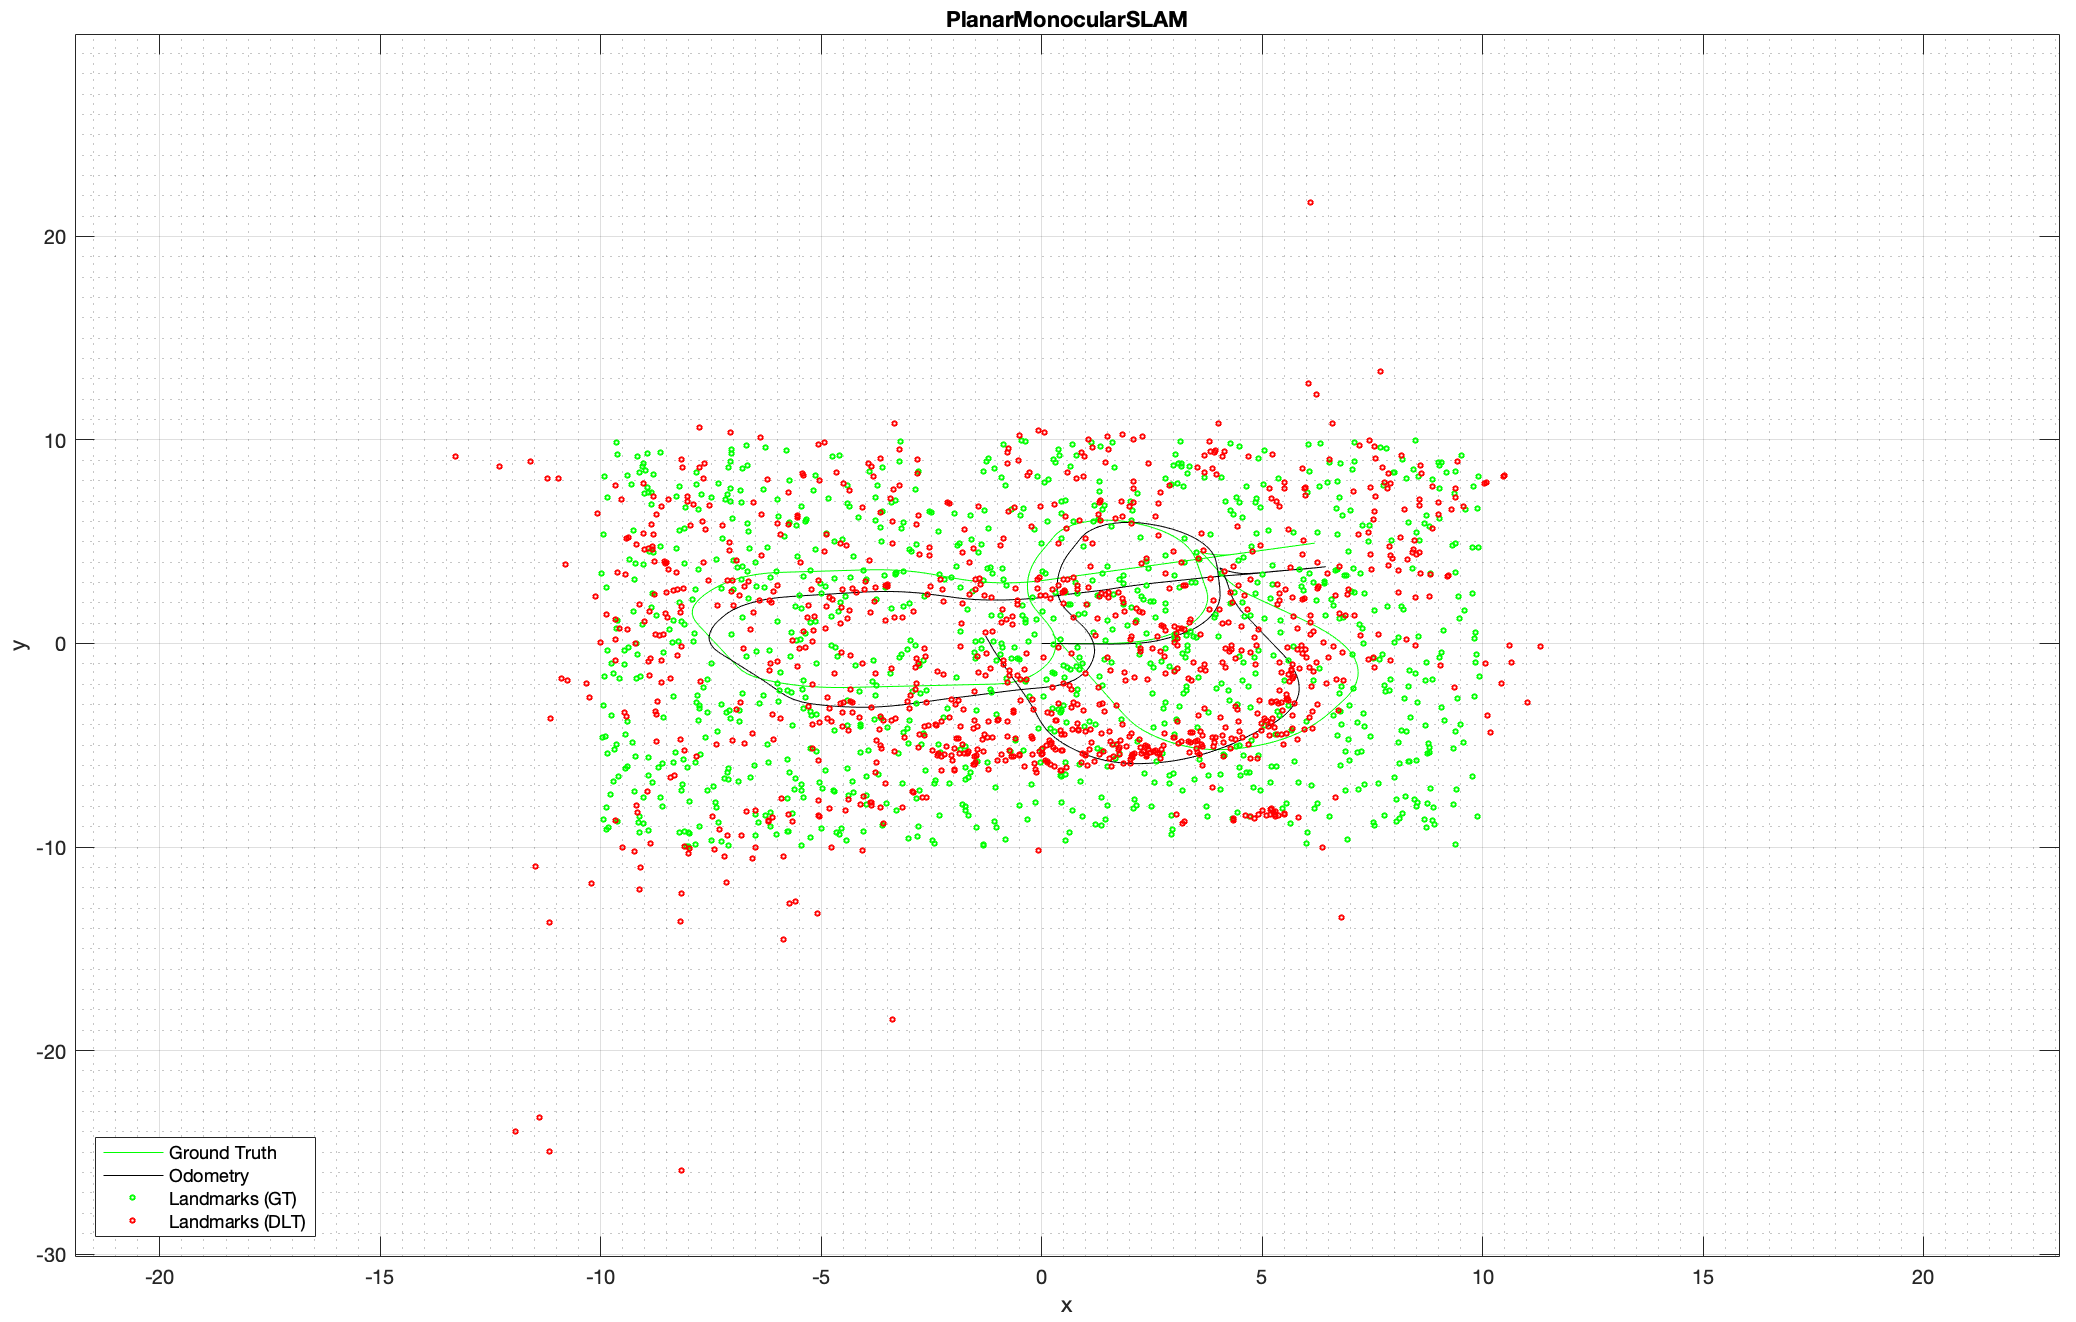
\includegraphics[width=\textwidth]{images/dlt-init.png}
    \caption{Initial reconstruction of the landmarks using the DLT algorithm.}
    \label{fig:dlt-init}
\end{figure}

\section{Least Squares}
Once the position of each landmark has been initialized, a least squares
algorithm optimizes the given constraints. In particular, pose-pose constraints
have been used from the odometry, expressing the pose of each robot with
respect to the previous pose in the trajectory, and pose-landmark constraints
have been used from the camera measurements, where each landmark is expressed
in the image coordinates of the corresponding pose.

The implementation of the least squares follows a similar implementation of the
total least squares shown during the lectures. The Jacobians have been computed
analitically and the algorithms has been executed for 15 iterations.

%\subsection{Pose-Pose Constraint}
%Stuff.

%\subsection{Pose-Landmark Constraint}
%Stuff.

%\section{Results}
Fig. \ref{fig:slam-ls} shows the result of the least squares algorithm at
the end of its execution. Notice that the ground truth of the trajectory is
completely covered by the solution as well as most of the landmarks. As
already introduced before, the landmarks which did not converge are those who
were initialized with a value too far away from the right one.
\begin{figure}
    \centering
    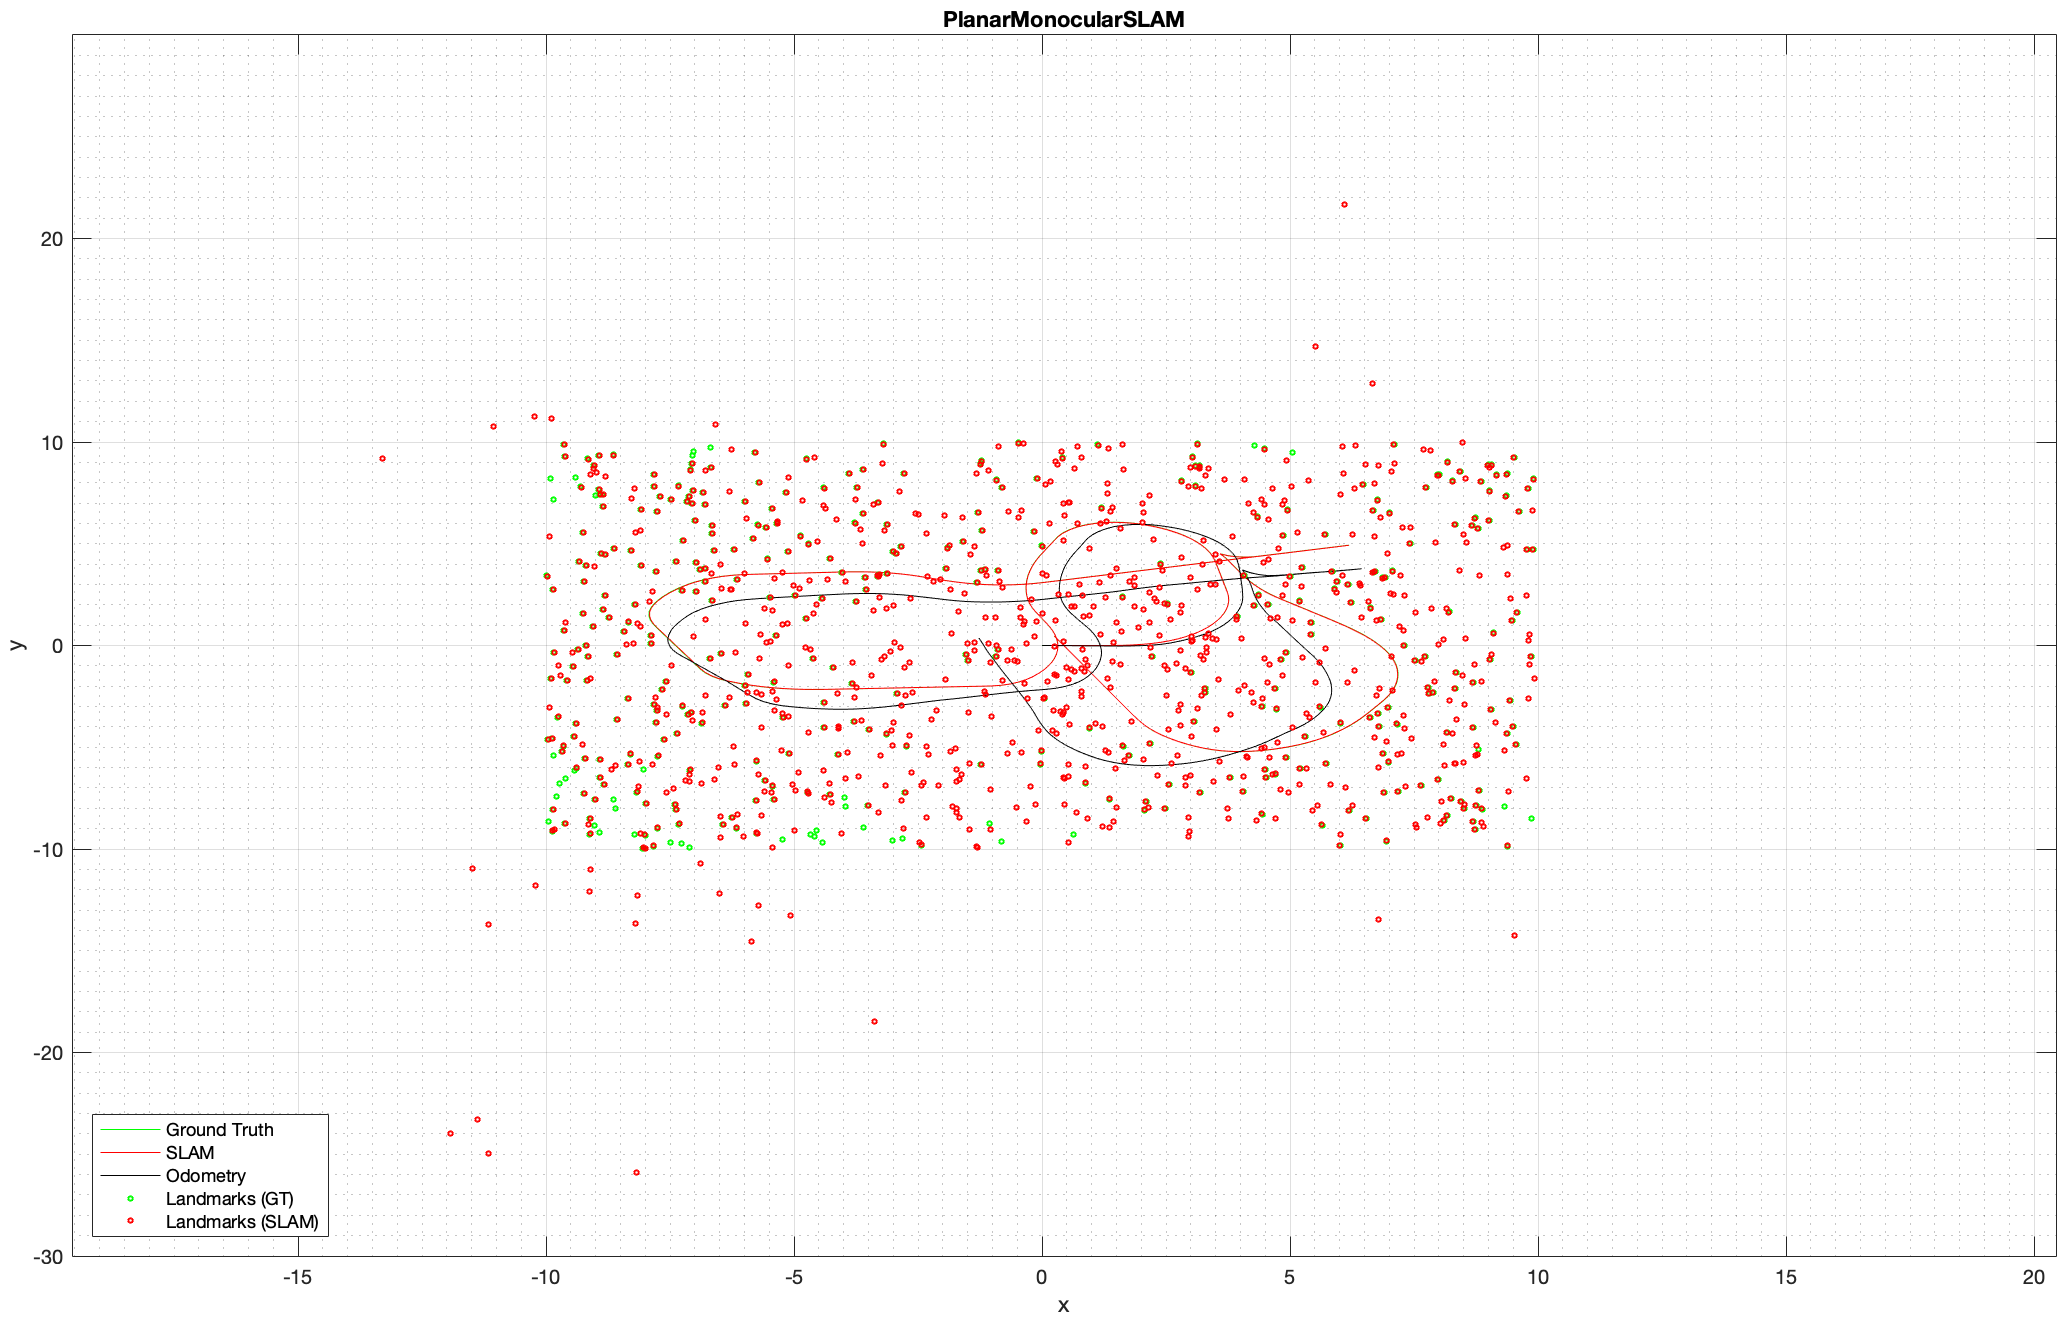
\includegraphics[width=\textwidth]{images/slam-ls.png}
    \caption{Result obtained after the execution of the least squares
        algorithm on pose-pose (odometry) and pose-landmark (projective)
        constraints.}
    \label{fig:slam-ls}
\end{figure}

Fig. \ref{fig:chi} shows how chi changes for both pose-pose (odometry) and
pose-landmark (projective) constraints.

\begin{figure}
    \centering
    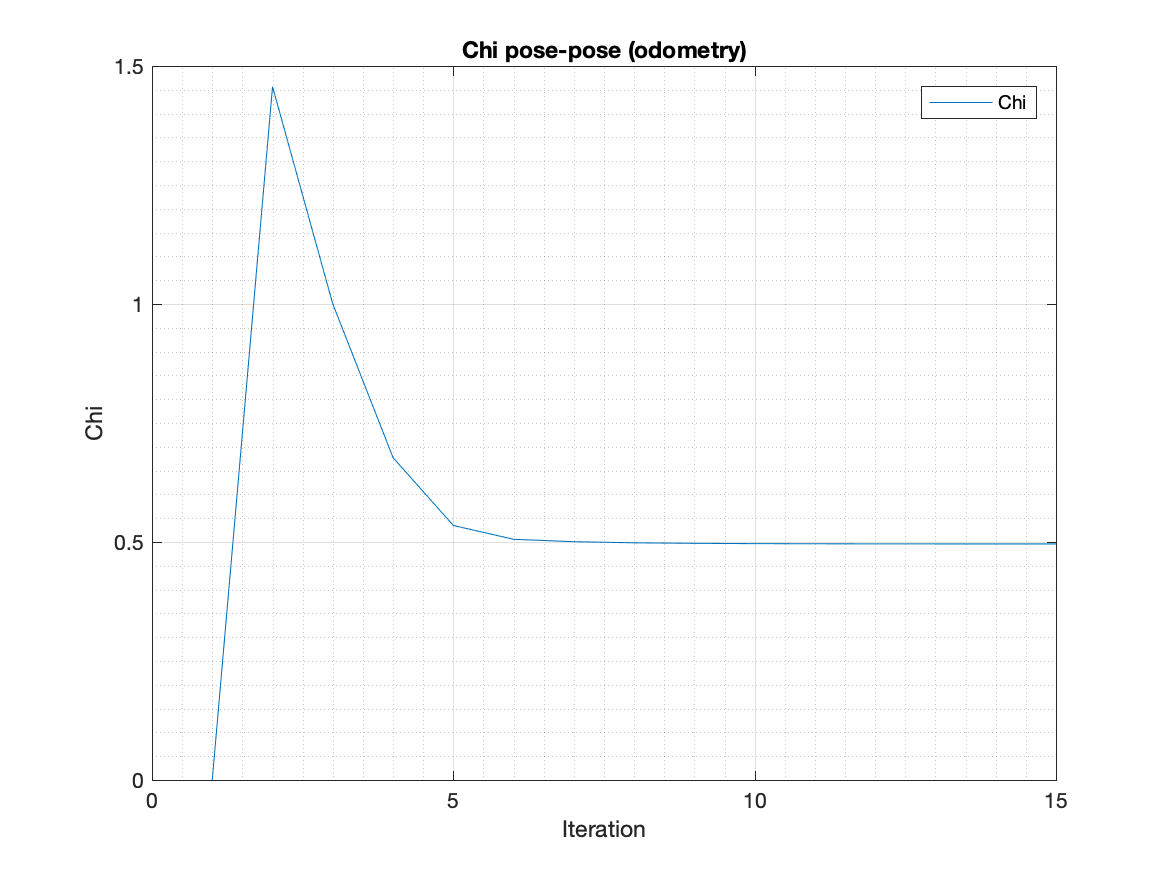
\includegraphics[width=0.495\textwidth]{matlab/chi-pose-pose-odom.png}
    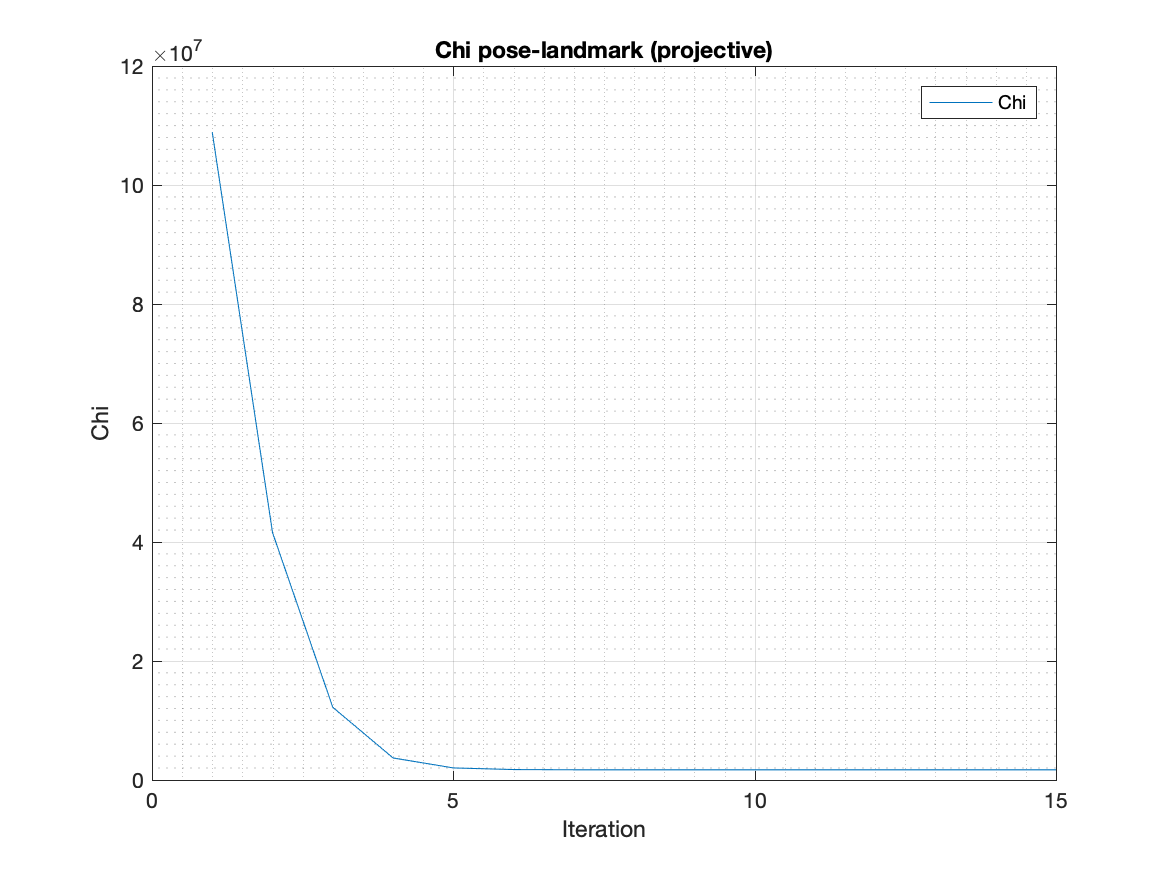
\includegraphics[width=0.495\textwidth]{matlab/chi-pose-landmark-proj.png}
    \caption{Behaviour of Chi through each iteration of least squares. On
        the left pose-pose constraints (odometry), on the right pose-landmark
        constraints (projective).}
    \label{fig:chi}
\end{figure}

\section{Conclusion}
The implemented algorithm obtained great results in both the trajectory and
the map reconstruction. Nevertheless, it can be improved a lot by better
exploiting the given data. More pose-pose constraints can be added by
triangulating the poses (e.g. by using the 8-point algorithm), landmark-landmark
constraints could be added by considering, again, the given relations between
poses and landmarks due to the camera. The k-d tree implementation can be
improved by considering that the landmarks should be initialized with the
appearance of the landmarks coming from the measurements. In the end, the
least squares implementation is not exploiting the sparsity of the matrix $H$,
which should boost the performances and massively decrease the amount of memory
used in this step.

\clearpage
\bibliographystyle{ieeetr}
\bibliography{bibliography}

\end{document}
